
%%%%%%%%%%%%%%%%%%%%%%%%%%%%%%%%%%%%%%%%%%%%%%%%%%%%%%%%%%%%%%%%%%%%%%%%%%%%%%%%
%2345678901234567890123456789012345678901234567890123456789012345678901234567890
%        1         2         3         4         5         6         7         8

%\documentclass[letterpaper, 10 pt, conference]{ieeeconf}  % Comment this line out if you need a4paper

\documentclass[a4paper, 10pt, conference]{ieeeconf}      % Use this line for a4 paper
\usepackage[T1]{fontenc}
\usepackage[utf8]{inputenc}
\usepackage[english]{babel}
\IEEEoverridecommandlockouts                              % This command is only needed if
                                                          % you want to use the \thanks command

\overrideIEEEmargins                                      % Needed to meet printer requirements.

% See the \addtolength command later in the file to balance the column lengths
% on the last page of the document

% The following packages can be found on http:\\www.ctan.org
%\usepackage{graphics} % for pdf, bitmapped graphics files
%\usepackage{epsfig} % for postscript graphics files
%\usepackage{mathptmx} % assumes new font selection scheme installed
%\usepackage{times} % assumes new font selection scheme installed
\usepackage{amsmath} % assumes amsmath package installed
%\usepackage{amssymb}  % assumes amsmath package installed
\usepackage{algorithm}% http://ctan.org/pkg/algorithm
\usepackage{algpseudocode}% http://ctan.org/pkg/algorithmicx
\usepackage{graphicx}
\usepackage{moreverb}

\title{\LARGE \bf Project Report \\ EDAN70 Project in Computer Science \\ Intelligent Systems \\ Classifying Laser Range Data "Images" \\ Supervisor: Elin Anna Topp}
\date{\today}
\author{Fredrik Paulsson \\ dat11fp1@student.lu.se \and Shan Senanayake \\ dat11sse@student.lu.se}


\begin{document}
\maketitle
\thispagestyle{empty}
\pagestyle{empty}


%%%%%%%%%%%%%%%%%%%%%%%%%%%%%%%%%%%%%%%%%%%%%%%%%%%%%%%%%%%%%%%%%%%%%%%%%%%%%%%%
\begin{abstract}
This report documents a project in which we developed a classifier for laser range data "images". The classifier was based on machine learning meaning that the classifier identified measurements and classified them based on previosuly known classifications of measurements.

In the report we describe two approches to solve the problem of developing this classification. The different approaches works on different levels of abstraction, one based on individual points and one based on lines among the points. There was several problems with the classifier working among points while we had more success with the one working on points.

Because of time constraints we did not have much time to work the the second approch but in the report we list the results that we have produced and we also specify improvements that can be made in order for it to possibly work much better.


\end{abstract}


%%%%%%%%%%%%%%%%%%%%%%%%%%%%%%%%%%%%%%%%%%%%%%%%%%%%%%%%%%%%%%%%%%%%%%%%%%%%%%%%
\section{INTRODUCTION}

In this project we were to develop a classifier that takes as input laser range data and outputs a classification of the data. The classification may be \emph{door}, \emph{open space}, \emph{clutter} and maybe \emph{wall} and similar objects.

The goal was to implement the calssifier as a ROS node in C++ so that it could run online on a robot.

The project consists of several parts. The first part was to develop a parser for the laser range data that wrapped the data in suitable data structures as well as transforming the representation into a form that was easier to work with.

The second part was to develop and implement an algorithm that had the abillity to classify the laser range data. This algorithm were supposed to operate within the data structures that our parser had created.

The third part was to port the classifier into a ROS node and test it in an online environment running on the robot. 

During development we used laser range data that had been gathered in the past.

This report will serve as documentation of our project.

\section{Machine Learning}
We are both very interested in machine learning and therefore we decided to develop our classifier within the machine learning area of artificial intelligence.

The idea that we had was to combine both supervised and unsupervised learning for use in order to classify laser range data. The original idea that we had was based on manually classifying some measurements in order for the classifier to have a database to start with. When the classifier was to be used it was going to browse the database and find out which laser range data in the database that matched best with the measurement that was going to be classified. It was then going to give the new data the same classification as the data that matched best. We also visioned that the new classification might be added to the database in order for the robot to learn.

We had discussed and thought about having a threshold on how good the best match needed to be in order for it to be used. If that threshold was crossed the classifier would either be unable to give a classification, give an "unknown" classification or simply prompt a warning that the classification may be wrong. Also we thought about having a threshold on the match that was going to be even harder to accomplish than the threshold previosly introduced. This threshhold was simply going to control whether or not the new classification was going to be added to the database. This was for allowing a poor match to be successfully classified but not to extending the database with "bad" knowledge.

However, later on in the project we changed the approach from our original idea to switch to using decision trees instead. This new idea was based on identifying characteristics in the measurements and then use these characteristics in order to classify measurements. The advantage with this approach was that we raised the abstraction level of the classifier. Instead of working on individual points it worked on patterns recognized among the points.

\section{PARSER}
The offline data of measurements that we have used to test our classifier and based the supervised learning part on was given to us in a specific format. All measurements gathered in one run of the robot's laser range scanner is put into one single file called \emph{scans.dat}. Each single measurement is placed on its own line. Measurements were gathered with a frequency of 4-5 Hz according to our supervisor.

Each of these measurements had a specific format and each measurements starts with a header of 15 values and then a value for each point in the measurement. The laser range scanner works by emitting a certain number of laser beams which will be reflected in obejcts in the field of view of the scanner. The scanner will then calculate the distance to each reflection point resulting in a number of distances. In each measurements the number of points and the angle between the points are given. Effectively each point's coordinates is given in polar form.

Each measurement looks like the following:

\begin{verbatim}
<unknown> <unknown> <number_of_points>
<timestamp_seconds> 
<timestamp_microseconds>
<unknown> <unknown> <unknown> <unknown>
<unknown> <unknown> 
<angle_between_points>
<unknown> <unknown> <unknown>
<distance_in_meters>^<number_of_points>
\end{verbatim}

As can be seen there are a lot of unknown values that we do not know and that our supervisor could not explain to us. However, these values are not needed by us in this project. The most important values are the number of points, the angle between the points and for each point the distance to the point.

Directly parsing the above format of each mesurement yields polar coordinates. Polar coordinates are very hard to work with as they are not easily visualized or easily worked with. This made us constructing a transformation of these polar coordinates into our own cartesian coordinate system.

Our coordinate system is based on some basic principles. The robot is positioned at origin and is the front of the robot is along the y-axis. This is basically the standard way to transform between polar and cartesian coordinates. The only special this is that the angle for the polar coordinates is expressed from the starting point. However, the starting point may be located at different angles from the x-axis depending on the specific type of laser range scanner. Different scanners may have a different number of points, different angle between the points and differently sized fields of view. With field of view we mean the entire angle that the scanner scans. In order to manage this problem we chose to express the angle from the y-axis instead and thus replace the use of sinus and cosinus with each other in the standard transform and also to manage the sign of each coordinate.

Now that we had coordinates in a much more manageable represenation we could visualize the data for ourself and we could use standard mathematical formulas in order to work with each measurement. As we needed to manually classify measurements in order to feed these to the classifier as a starting ground it was vital that we could easily plot the measurements. This was easily done in Matlab or Octave when we had our cartesian coordinates. Figures \ref{human}, \ref{doorhalf}, \ref{doorfull} and \ref{chair} shows some example plots.


\begin{figure}
\centering
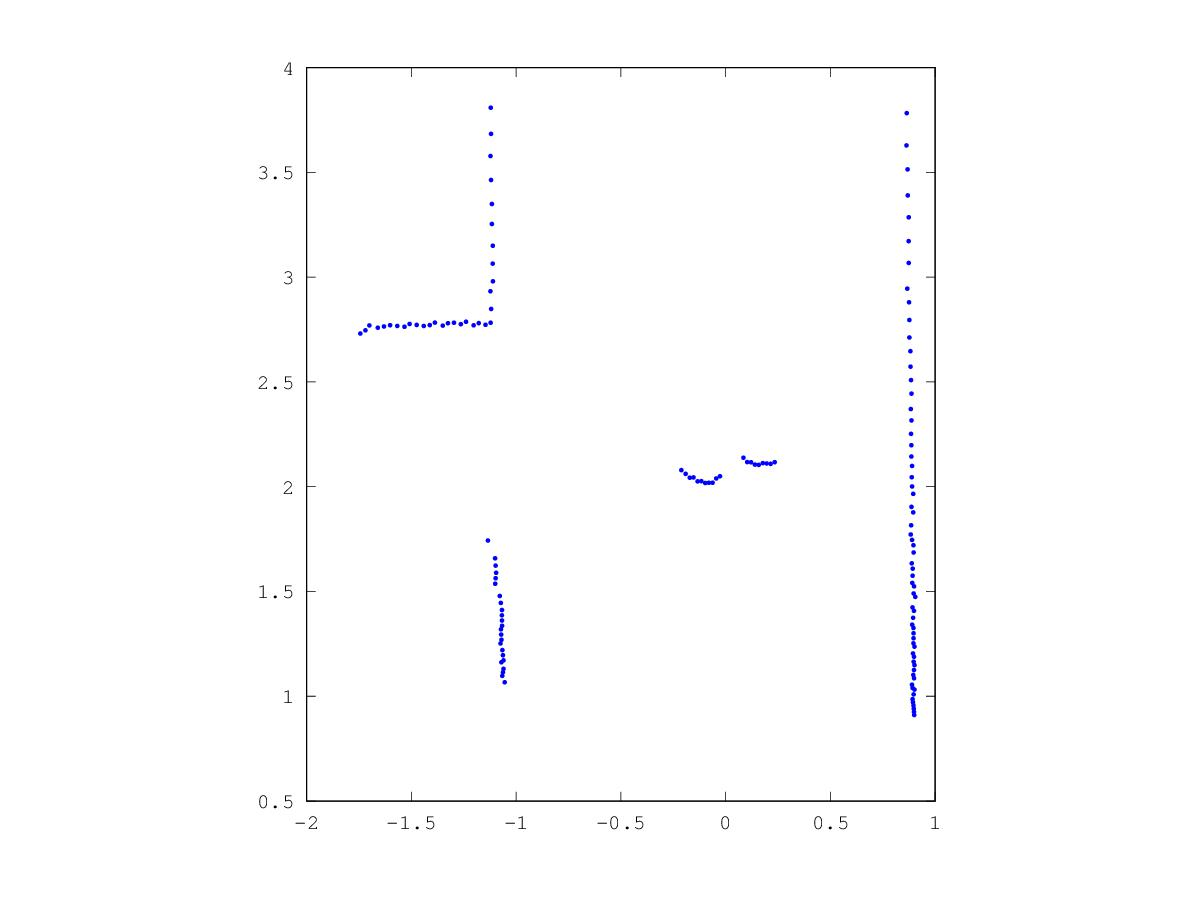
\includegraphics[width=0.5\textwidth]{presimg/human.jpg}
\caption{This plot shows a human standing in front of the robot in a hallway. The human legs are clearly visible in the center of the plot.}
\label{human}
\end{figure}

\begin{figure}
\centering
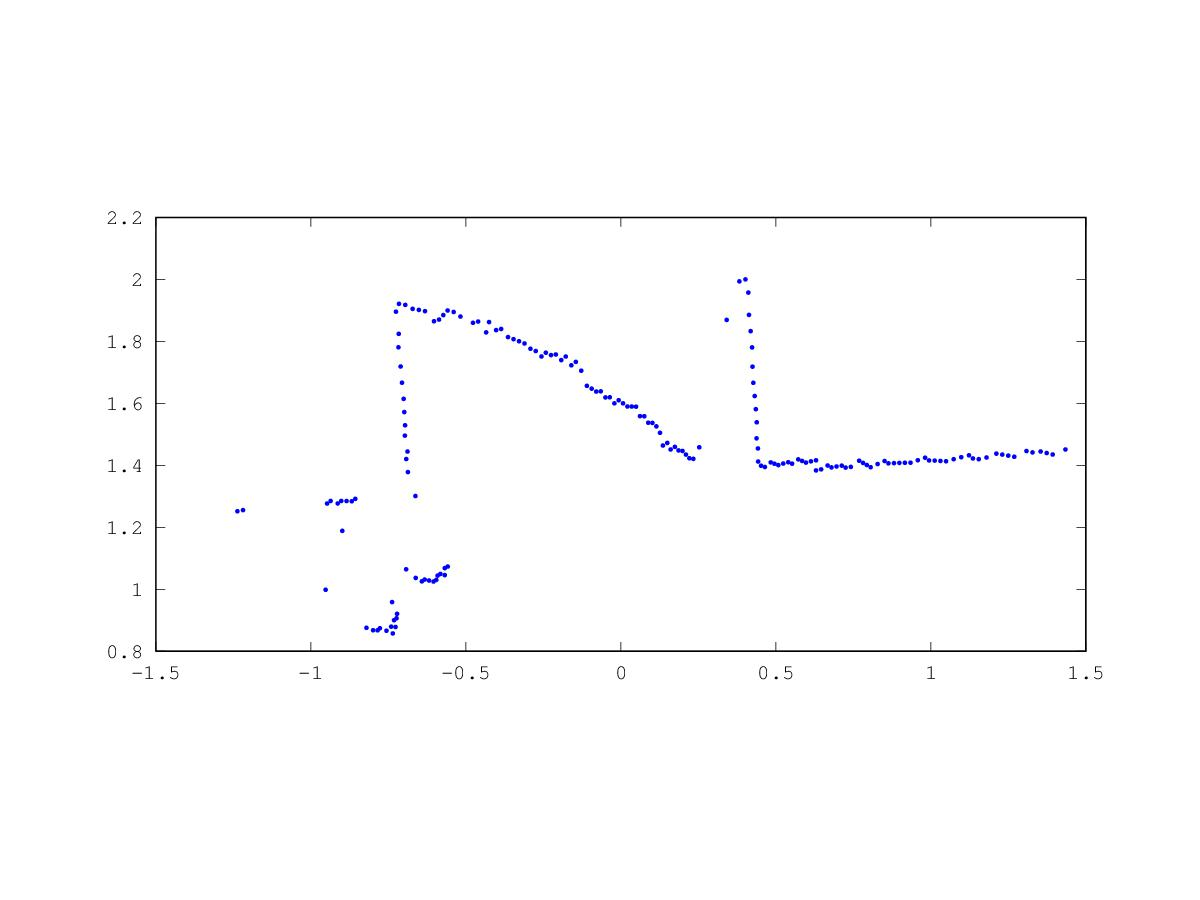
\includegraphics[width=0.5\textwidth]{presimg/doorhalf.jpg}
\caption{This plot shows a door that is half open. There is also a human standing in front of the door to the left.}
\label{doorhalf}
\end{figure}

\begin{figure}
\centering
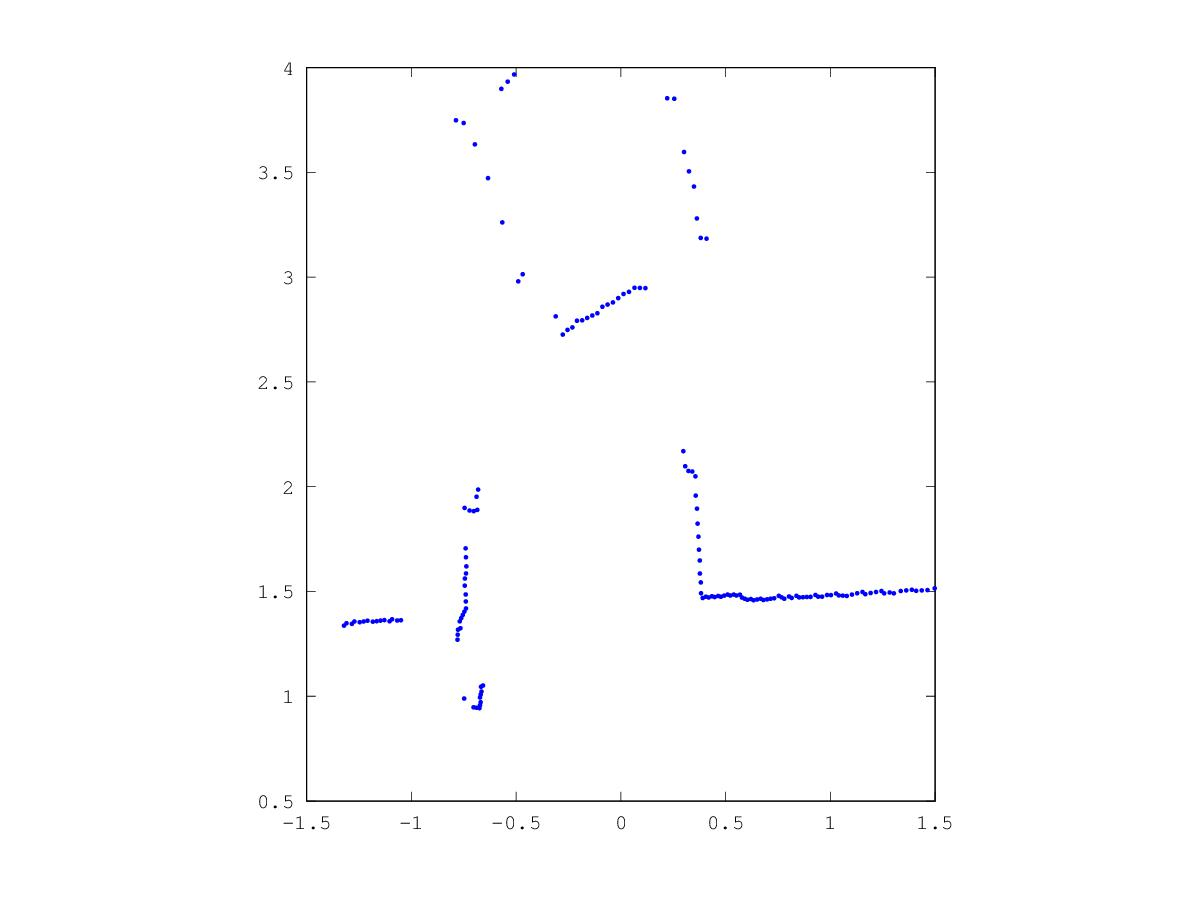
\includegraphics[width=0.5\textwidth]{presimg/doorfull.jpg}
\caption{This plot shows the same door as the plot above but now the door is fully open. Now some clutter is shown from inside the room.}
\label{doorfull}
\end{figure}

\begin{figure}
\centering
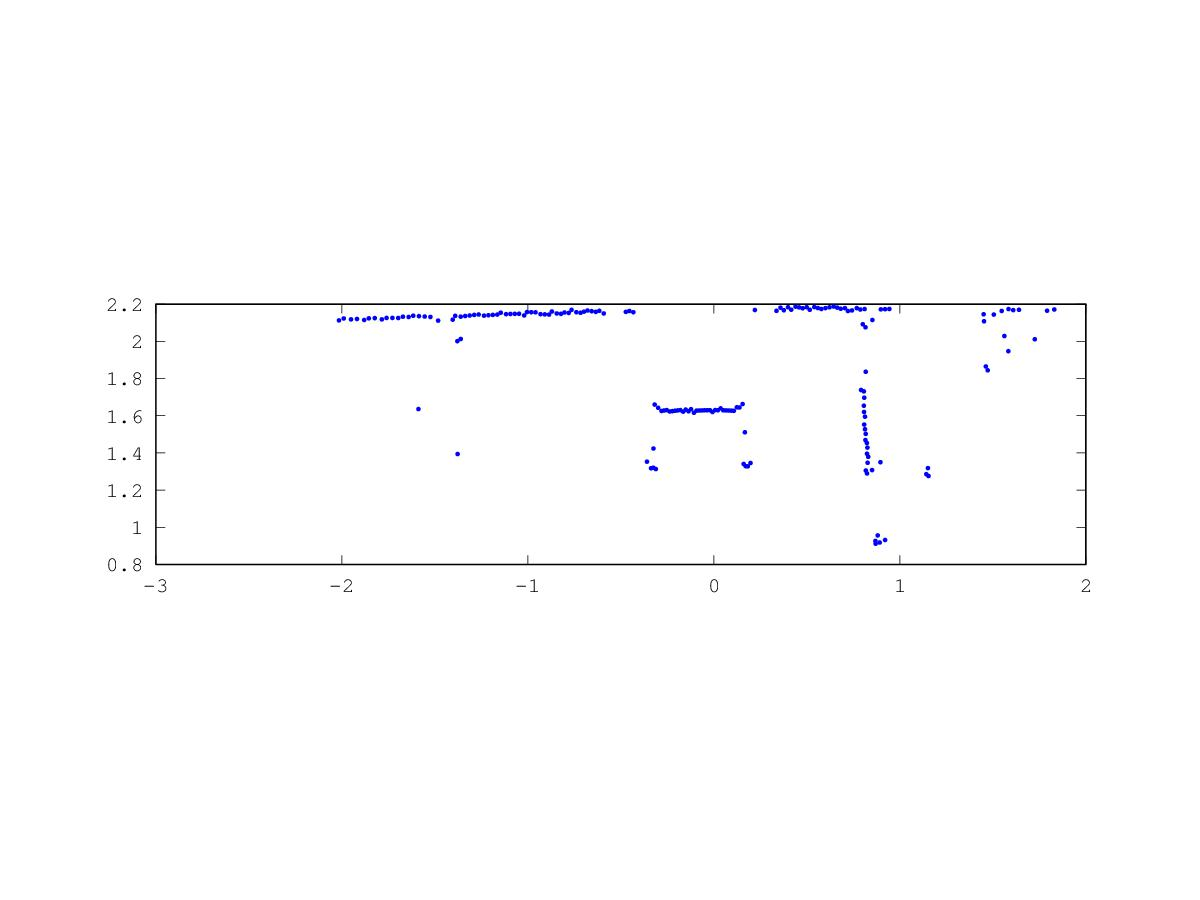
\includegraphics[width=0.5\textwidth]{presimg/chair.jpg}
\caption{This plot shows the robot standing in the middle of a room facing a wall. Right in front of the robot a chair is positioned.}
\label{chair}
\end{figure}

\section{ALGORITHM}
In this section we will explain all of the algorithms we used and how they were implemented. 

We hade two different approaches when trying to figure out a way to represent the data in a form where we could easily apply some form of machine learning on it. This was the biggest challange we had to overcome in the project. 

\subsection{Interpolation and Comparison}
After transferring the data to a form which we could more easily differentiate the characteristics of the data we decided to try a interpolation approach. This approach consisted of interpolating the data points to get a 'figure' of some sorts which we could use as a characteristic for a classifier.

The interpolation is mainly used to get an evenly distributed set of point which we could use to directly compare with another set of points to see how much error they have.

The idea behind this approach was to store measurements and their respective classifications in some sort of database. When the classifier then receives a measurement to classify the classifier would iterate over the database and using the interpolation to directly compare the new measurement with all measurements stored in the database. The classification of the best match in the database would then be assigned to the new measurement. And finally the new measurement and it's classifaction were to be stored in the database.

This idea would combine both unsupervised and supervised machine learning. The supervised learning came into play because there would need to be a databse from the start. The classifications contained in this databse had to be manually classified by us. The unsupervised learning takes place because the classifier extends it database on each run.

Possibly, the above algorithm could incorporate thresholds and a default classification. Essentially this means that if there did not exist a match that had an error less than the threshold the clasifier might assign the classification unknown or something simillar. This acts as the default classification and if it is used the algorithm should not add the newly classified measurement to it's database.

\subsubsection{Implementation}
We decided to start the implementation with a simple linear interpolation algorithm, pseudocode is found in algorithm \ref{lerp}.

\begin{algorithm}
  \caption{\label{lerp}Simple lerp}
  \begin{algorithmic}[1]
      \State \texttt{Dataset S}
      \State \texttt{Number of points N}
      \State \texttt{Distance increment $d$ = Total distance / N}
      \State \texttt{$i = 0$}
      \State \texttt{Point lower,upper in S}
      \State \texttt{Array of points A}
      \While{\texttt{$i <$ Total distance}}
      	\If{$lower < i < upper$}
      		\State A.add(Calculate point of ($i$));
      	\ElsIf{$lower == i$}
      		\State A.add($lower$)
      	\ElsIf{$upper == i$}
      		\State A.add($upper$)
      	\Else
      		\While{$i>higher$ and S.End}
      			\State \texttt{increment $lower$}
      			\State \texttt{increment $upper$}
      		\EndWhile
      	\EndIf
      	\State \texttt{$i += d$}
      \EndWhile
      \Return \texttt{A}
  \end{algorithmic}
\end{algorithm}

This algorithm is heayvly influenced by a simple linear spline interpolation \cite{interpolation}. The \texttt{Number of points N} variable is an input to decide how many points one wants to represent the Dataset in. The \texttt{distance increment d} is used to check out where the next point should lie. \texttt{Total distance} is the total distance if you walk through all the points in the dataset (Just like connecting the dots). The \texttt{$lower < i < upper$} is to check if the distance $i$ lies inbetween the \texttt{lower} and \texttt{upper} points. \texttt{Calculate point of($i$)} is used to calculate the point that should lie on that distance.

\subsection{Line finding}
\label{sec:line_find}
The other approach to representing data was a bit more of an abstract apporach. Instead of comparing the dataset against each other directly by using interpolation we decided to find characteristics within the dataset itself. 

The line finding algorithm does exactly what it says it finds lines in a given dataset, and given thease lines we can decide different characteristics. For instance the characteristics we chose to determine doors was how many lines there are, what is the mean length of thease lines, how many are parallel against each other and finally, how many are perpendicular against each other.

The thought process behind this stems from this article \cite{legfinding} which handles how to detect legs in laser range data. We have a simple line finding algorithm, that draws a line between the first two points in a set and then uses this line to check if the next line between the first and the third point are in a given bounding box. The bounding box is determined by the simple line equation $y = kx + m$ where the upper and lower limit is determined by $y = kx + m \pm err$. 

To not make the first k-value to set the entire lines value we have decided to tweak the k-value depinding on the amount of points already evaluated. This is done by calculating the weight each point has (in essence the effect) on the overall line and then updating the k value depending on the weight.

To reduce noise and wrong line finding we have determined to qualify for a line in the dataset it has to have more than 3 points from the dataset and the length of the line has to be greater than 0.25 m.
\subsubsection{Implementation}
The pseudocode for the Line finding algorithm can be found in algorithm \ref{lineFinding}.

\begin{algorithm}
  \caption{\label{lineFinding}Line finding}
  \begin{algorithmic}[1]
      \State \texttt{Dataset S}
      \State \texttt{Error limit E}
      \State \texttt{Point start in S}
      \State \texttt{Array of lines A}
      \While{\texttt{S has unevaluated points}}
      	\State \texttt{Point p1 in S}
      	\State \texttt{$k$ = Calculate K Of (start,p1)}
      	\State \texttt{$d$ = Distance of (start,p1)}
      	\While{Is a valid line}
      		\State \texttt{Point p2 in S}
      		\State \texttt{$lower$ = calculate lower of line (start,$k$,E)}
      		\State \texttt{$higher$ = calculate higher of line (start,$k$,E)}
      		\If{Check if point is in bound ($lower$,p2,$higher$)}
      			\State \texttt{$new_k$ = calculate k of (start,p2)}
      			\State \texttt{update k ($k$,$new_k$)}
      			\State \texttt{p1 = p2}
      		\Else
      			\State \texttt{break inner loop}
      		\EndIf
      	\EndWhile
      	\If{line is valid($k$,start)}
      		\State \texttt{A.add($k$,start)}
      	\EndIf
      \EndWhile
      \Return \texttt{A}
  \end{algorithmic}
\end{algorithm}

Just as explained in section \ref{sec:line_find} the line finding algorithm takes a thick line and adjusts the k-value for each point that fits in the line. The function \texttt{Caluculate k of (start,p1)} just calculates the $k$ value of two points accordning to the regular linear equation $k = \frac{\delta y}{\delta x}$, the functions \texttt{calculate lower of line} and \texttt{calculate higher of line} calculates how thick the lines which checks errors are. Similair the function \texttt{Check if point is in bound} simply check if the point \texttt{p2} is within the margin of error. The most interesting function is \texttt{update k} which calculates a new $k$-value depending on the previous and how many points we already have evaluated. The weight is caluclated by $w = \frac{1}{number of points already evaluated}$ and the new $k$ is caluculated according $k = (1-w)*k + w*(new_k)$.

\subsection{Decision Tree}
When we had identified line characteristics in our measurements as described above we had raised the level of abstraction in our data. Instead of comparing point by point against each other in order to identify patterns we could now decide based on the characteristics to which class the given measurement belongs. After some research we deduced that a decision tree was a good way to proceed within the machine learning area of artificial intelligence.

The great part of decision trees that attracted us was the fact that the input to the algorithm can be several very abstract variables. The variables can be both discrete values or real values. Decision trees also has one big advantage and that is that they are very robust against errors and noise in the training examples \cite{ml3}. The measurements that we have used can be very noise so decision trees seemed like it would work very well.

Our classification problem were going to consist of more than simply two classes. However, the decision tree outputs only a boolean, yes/no, classification for each measurement \cite{ml3}. The way we solved this problem was to use a so called one-vs-rest classifier \cite{praml}. This essentially means that we train one classifier, or in our case one decision tree, for each class that we want be able to classify. The output from each of these classifiers is simply a yes if the measurement is part of that class or no if the measurement is not part of that specific class but may be a member of the others.

\subsubsection{Implementation}
The algorithm that generates our decision tree is the well-known ID3 algorithm. Our exact implementation is based on the description and structure presented in \cite{aima}, however, a more formal presentation can be found in \cite{ml3}. As discussed in \cite{aima} our algorithm selects the attributes to split on by their information gain. In order to use real continuous values for the branches we use splitpoints.

However, the process of acquiring good splitpoint values we use the process described in \cite{ml3}. The process of selecting a good splitpoint for a certain attribute is by sorting the examples by the attribute. The next step is to find all pairs of adjacent examples in the sorted list that differs in their classifications. For each pair, one calculates the information gain of the mean of the pair's values. Then it is simply to select the pair whose mean value maximizes the information gain.

Even though decision trees that works with contionous values on the attributes are called regression trees, our tree is not a regression tree. We never switch over to do any kind of regression. For every attribute we simply have a splitpoint that separates the subtree in two branches, a so called binary split \cite{aima}.

\section{RESULTS}

\subsection{Parser}
The result for the parser is pretty straightforward. Figures \ref{human}, \ref{doorhalf}, \ref{doorfull} and \ref{chair} have all been plotted using the cartesian coordinates that our parser have parsed and transformed. In all these plots the robot is located at origin and is heading forward along the y-axis. Furthermore, in all plots we have narrowed the field of view to 90 degrees and we only include points within 4 meters of the robot in order to provide a more clear plot with minimum noise. However, even though we have limited the number of points plotted our parser is able to include every point made by the laser range scanner.

\subsection{Interpolation and Comparison}
While implementing this algorithm we encountered several practical problems and eventually we relaized that this was not going to work very well. Therefore, we abandoned this approach and starting researching other ways resulting in the second idea explained above. Thus, we have no results to provide from this algorithm other than we never got it working.

\subsection{Line finding}
This is the main algorithm we are using to represent datasets. 

!!!TODO!!! Här måste vi lägga in biler på linjer som vi identifierat

\subsection{Decision Tree}
!!!TODO!!! Exempel träd

\section{DISCUSSION}

\subsection{Parser}
The parser was relatively simple to develop, based on standard transformations from polar coordinates to cartesian coordinates. The only problems we had was specific to the laser range scanner. At first we assumed that points was listed in clockwise order but it was actually listed in counter-clockwise order according to mathematical notation.

The biggest problem to overcome with the parser was that we only knew the angle between two adjacent points and not the absolute angle for each point. This led us to express the angle for each point as the absolute angle from the first point. Since we wanted to make our parser work for any laser range scanner we could not assume where the first point was located. Thus, our solution was to express the angle for each point as the angle between the point and the y-axis that we were to create. This was possible since we could calculate the field of view for the scanner, we knew that the y-axis was located exactly in the middle of the field of view. But, expressing the angle in this way meant that sinus and cosinus had to replace each other in the transformations as well as we had to explicitly manage the sign of the coordinates.

However, other than this we did not have any major trouble with the parser.

\subsection{Algorithms}

\subsubsection{Interpolation and Comparison}
A stated above we realized that this algorithm would not work and we never finished the implementation. There were several reasons for this. First of all, the datasets that we recevied from our parser were all simply a set of points. Potentially the different measurements that we were going to store could come from different laser range scanners. Thus, a certain number of points could describe two differently sized fields of view. This is the main reason why we introduced interpolation so that we could compare the same points on the two different measurements.

The next problem to solve was that we realized that in principle we needed to overlay each measurement on the other and then glide them over each other in order to minimize the error between them. However, even the slightest shift could introduce huge errors. We never came up with a solution to this problem and instead we chose to abandon this approach and research other ways of classifying measurements.

\subsubsection{Line finding}
There are quite a lot of parameters that require tweaking in the line finding algorithm. The reasoning behind these parameters will be explained here.

\begin{description}
\item[0.25 m lenght of line:] \hfill \\ This parameter was chosen so as to not mistake feet for line, since on quite a lot of the datasets a couple of feet will turn up and most of the furniture has legs as well.
\item[more than three points:] \hfill \\ To determine a line more than 3 points has to be chosen, this parameter was chosen to be more than three so that the algorithm does not draw lines over huge gaps which consists of 2-3 points.
\end{description}

!!!TODO!!! Här måste vi diskutera mer, måste skriva att vi inte hade tid


\subsubsection{Decision Tree}
!!!TODO!!! Måste skriva att vi inte hade tid att få det bra

\subsection{Improvements}
There are several improvements that we have thought about in this project. The most obvious ones are the things we did not have time to implement. Furthermore, there are some improvements that we have philosophized about.

In order for our classifier to work as it was intended, to identify different types of objects, we need to implement the one-vs-rest classifier as discussed above. As stated above we did not have time to implement more than one classifier. Thus, the improvement is to train several more decision trees to be used in the classifier by combining them using the one-vs-rest technique.

Another clear improvement is to implement more attributes and characteristics to detect in the measurement. The idea here is to use more than 4 attributes that can be gathered from the lines. Possibly we could use attributes such as the number of corners, number of corners that mirror each other and similar attributes. Also, an obvious improvement here is to extend the attributes to not just lines but to other patterns. For example, circles, rectangles and other shapes could be identified and suitable abstract attributes involving these shapes could be used as input to the decision trees.

A nice feature to have in the classifier is unsupervised learning. This improvment can be quite easily implemted by regenerating each decision tree once a new classifiaction has been made. The classification would in this case be added to the examples that is used to generate the trees.

The last obvious improvement is to implement the classifier as a ROS node so that it could be used online on the robot. This was part of our original goal with project but unfortunately we did not have time to fulfill that specific goal.

These improvements are those that would make the classifier somewhat useful if combined together. The robot could travel around and at specific intervals it could output a classification of what it currently sees. For example, if it detects a door it outputs that fact and if it detects a human it would state that. The classifications can be sent to the programs that dictate movement so that, for example, a human would suddenly appear, the robot would stop.

However, we do have some improvements that we believe might increase the performance of the classifier.

Firstly, the line finding algorithm could be exchanged for a much better algorithm that really identifies the lines we have always wanted to identify. The main problem with our algorithm is that it is directly dependent on the index of each point in the measurement. We strongly believer that this improvement would have a major impact on the perfomance of the classifier as it exists now.

Secondly, we have thought about another improvement which stems direclty from the fact that our initial approach failed. The problem was that we worked with individual points. The success came when we instead looked at lines and essentially raised the level of abstraction. Thus, we have philosophized about increasing the level of abstracion even further and introduce more layers to the classifer. For example, we use one classifier that looks at characteristics of lines and determine if certain shapes occur. One classifier could identify rectangles another triangles and so forth. Then the classifiers that actually detects doors, humans, open spaces e.t.c. base their decisions  on the output of these intermediate classifiers. This improvement is something we have just fantasized about and we can not in any way predict how the perfomance would be effected but it would be very interesting to test.

\section{CONCLUSION}
During this project we have learned several lessons. Most of the lessons have come from the fact that we did not have a good idea of how to approach the problem in the beginning. Therefore, we attempted one approach that eventually proved to be to difficult to solve. However, in the end we did find an approach that we believe in but because we did not have much time left we could not implement is as fully as we would have liked.

We learned quite late in the project that it was far better to raise the abstraction of the problem. This was hinted to us earlier in the project by our supervisor but we had no idea of how to approach the problem in that way. It was not after we had realized that the first approach was a failure that we were forced to make further research in order to find our next approach which made use of a higher abstraction level. It was here that we gained most knowledge, we realized that we could actually use decision trees to do pattern recognition. This was something that we would never have come up with from the beginning. However, even though we had found an approach that seemed pretty good there was not much time left before the end of the project. Therefore, we could only implement the simplest possible solution that actually yielded some result. The results were not astonishing but we believe that if the improvements listed above were to be implemented the results would be better.

The biggest pitfalls in our project was that we did not put as much effort into research as we should have, at least not in the beginning. It was not until our second research phase that we actually found something we could use. However, we made one big error and that was to implement our own line finding algorithm. Had we done research on that we would have produced much better results. The biggest reason for us not doing this research was because of the limited time we had left.

The main conclusion of this project is that it is better to approach this problem by looking at a higher level than on idividual points. This meant that an algorithm could take pretty abstract attributes as input in order to solve the problem.

We did not manage to meet all our goals and this was primarily because of the limited time. We would like to have been able to classify several different kinds of objects as well as being able to run the classifier online on the robot using ROS. We would also had liked to use unsupervised learning to let the clasifier improve on itself. however, these improvements have been discussed in this report.




%%%%%%%%%%%%%%%%%%%%%%%%%%%%%%%%%%%%%%%%%%%%%%%%%%%%%%%%%%%%%%%%%%%%%%%%%%%%%%%%



%%%%%%%%%%%%%%%%%%%%%%%%%%%%%%%%%%%%%%%%%%%%%%%%%%%%%%%%%%%%%%%%%%%%%%%%%%%%%%%%



%%%%%%%%%%%%%%%%%%%%%%%%%%%%%%%%%%%%%%%%%%%%%%%%%%%%%%%%%%%%%%%%%%%%%%%%%%%%%%%%
%\section*{APPENDIX}

%Appendixes should appear before the acknowledgment.

%\section*{ACKNOWLEDGMENT}

%The preferred spelling of the word �acknowledgment� in America is without an �e� after the �g�. Avoid the stilted expression, �One of us (R. B. G.) thanks . . .�  Instead, try �R. B. G. thanks�. Put sponsor acknowledgments in the unnumbered footnote on the first page.



%%%%%%%%%%%%%%%%%%%%%%%%%%%%%%%%%%%%%%%%%%%%%%%%%%%%%%%%%%%%%%%%%%%%%%%%%%%%%%%%

%References are important to the reader; therefore, each citation must be complete and correct. If at all possible, references should be commonly available publications.



\begin{thebibliography}{}
\bibitem{interpolation} here goes interpolation source

\bibitem{legfinding}Xavier, Joao. Pacheco, Marco. Castro, Daniel. Ruano Antonio. Nunues, Urbano. Fast Line, Arc/Circle and Leg Detection from Laser Scan Data in a Player Driver, http://miarn.sourceforge.net/pdf/a1738b.pdf
\bibitem{ml3} Mitchell, Tom M. Machine Learning. 1997. Chapter 3.
\bibitem{praml} Bishop, Christopher M. 2006. Pattern Recognition and Machine Learning. Chapter 4, section 1.2.
\bibitem{aima} Russel, Stuart. Norvig, Peter. Artificial Intelligence: A Modern Approach. Third edition. 2010. Chapter 18. 
\end{thebibliography}




\end{document}
